% Reports (up to ~2500 words including references, notes and captions–corresponds to ~3 printed pages in the journal) present important new research results of broad significance. Reports should include an abstract, an introductory paragraph, up to four figures or tables, and about 30 references. Materials and Methods should be included in supplementary materials, which should also include information needed to support the paper's conclusions.

% Main Text is not divided into sub-headings for Reports. 

% The manuscript should start with a brief introduction describing the paper’s significance. The introduction should provide sufficient background information to make the article intelligible to readers in other disciplines, and sufficient context that the significance of the experimental findings is clear. 

% \clearpage

Since early 2020, the CoViD-19 pandemic has presented an enormous challenge to humanity on many dimensions. The development of highly effective vaccines holds the promise of containment in the medium term. However, most countries find themselves many months---and often years---away from reaching vaccination-induced herd immunity.\comment[id=HM]{Cite some paper on herd immunity, maybe vaccine data} In the meantime, it is of utmost importance to employ an effective mix of strategies for containing the virus. The most frequent initial response was a set of non-pharmaceutical interventions (NPIs) to reduce contacts between individuals. While this has allowed some countries to sustain equilibria with very low infection numbers\comment[id=HM]{Cite Priesemann paper or other}, most have seen large ups and downs in their infection rates. Containment measures have become increasingly diverse and included testing, more nuanced NPIs, and contact tracing. Neither these policies' effect nor the influence of seasonal patterns or more infectious virus strains are well understood in quantitative terms. This paper develops a model incorporating all these factors. The framework allows to combine a wide variety of data in a timely fashion, making it useful to predict the effects of various interventions. We apply the model to Germany and show that rapid testing had the largest impact on the reduction in infections by XXX\% during the A weeks between X April and Y May.\comment[id=HM]{insert some useful numbers}. We conclude that rapid tests should play a large role...

At the core of our agent-based model are physical contacts between heterogeneous agents (Figure~\ref{fig:broad_model_description}).\footnote{We provide a detailed comparison to other approaches in \ref{sec:literature_review}. The model most closely related to ours is described in \citet{Hinch2020}.} Each contact between an infectious individual and somebody susceptible to the disease bears the risk of transmitting the virus. Contacts occur in the household, at work, at school, or in other settings (leisure activities, grocery shopping, medical appointments, etc.).\comment[id=HM]{Systemic relevance of work?} Some contacts recur regularly, others occur at random. Random contacts are typically assortative in age and geographical location. Empirical applications can take the population structure from census data and the types and frequency of contacts from diary data measuring contacts before the pandemic \citep[e.g.][]{Mossong2008}.\footnote{\citet{Hoang2019} provide access to multiple data sets on contact types and frequencies at \url{http://www.socialcontactdata.org/} covering countries from all continents except North America and Australia.} The dimensions are chosen so that the most common NPIs can be modeled in great detail by reducing the number of contacts in a particular setting or the risk of transmitting the disease for a type of contact. For example, a mandate to work from home will reduce the number of work contacts to zero for a fraction of the working population. Schools and daycare can be closed entirely, operate at reduced capacity including an alternating schedule, or implement mitigation measures like masking requirements or air filters.\comment[id=HM]{cite \url{https://science.sciencemag.org/content/early/2021/04/28/science.abh2939}} Curfews may reduce the number of contacts in non-work/non-school settings. In any setting, measures like masking requirements would reduce the probability of infection associated with a contact.

\begin{figure}[!tp]
    \centering

    \begin{subfigure}[b]{0.475\textwidth}
        \centering
        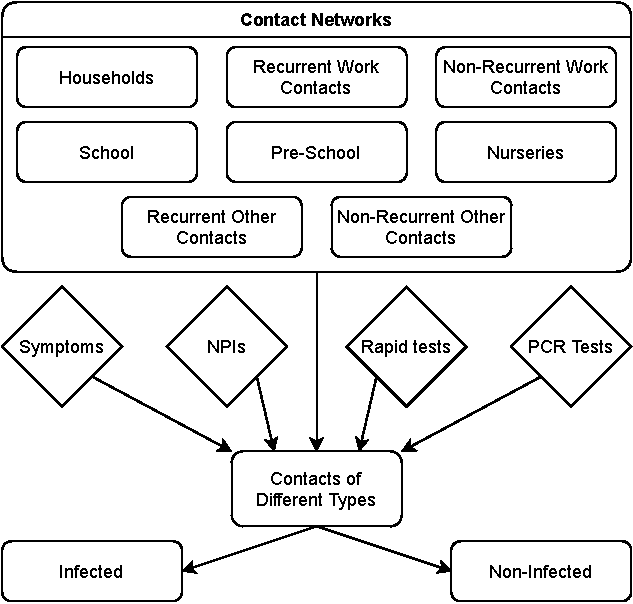
\includegraphics[width=\textwidth]{../figures/model-graph-top-left}
        \caption{{\small Model description}}
        \label{fig:broad_model_description}
    \end{subfigure}
    \hfill
    \begin{subfigure}[b]{0.475\textwidth}
        \centering
        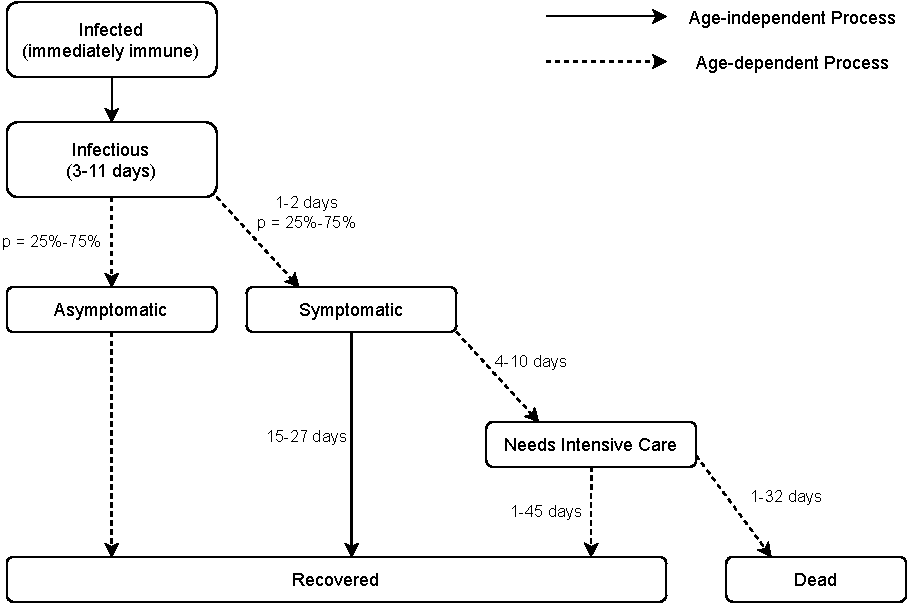
\includegraphics[width=\textwidth]{../figures/model-graph-top-right}
        \caption{Disease progression}
        \label{fig:disease_progression}
    \end{subfigure}
    \vskip3ex
    \begin{subfigure}[b]{0.475\textwidth}
        \centering

        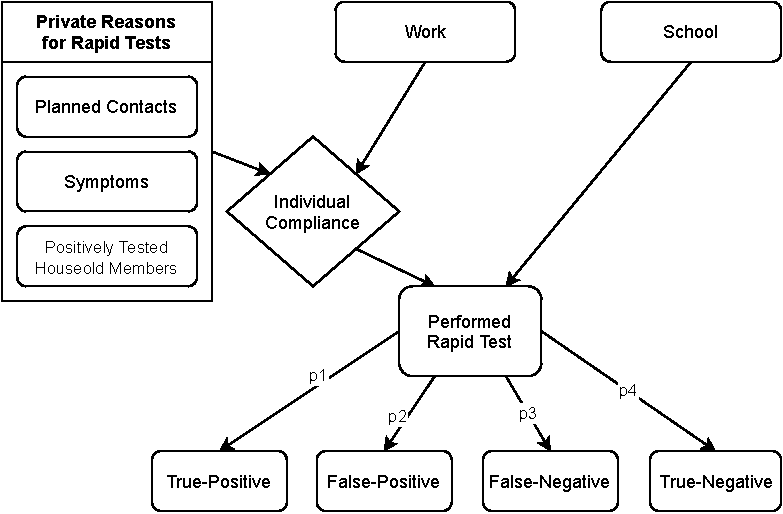
\includegraphics[width=\textwidth]{../figures/model-graph-bottom-left}
        \caption{{\small PCR and antigen tests}}
        \label{fig:pcr_antigen_tests}
    \end{subfigure}
    \hfill
    \begin{subfigure}[b]{0.475\textwidth}
        \centering

        Model for detected/undetected cases

        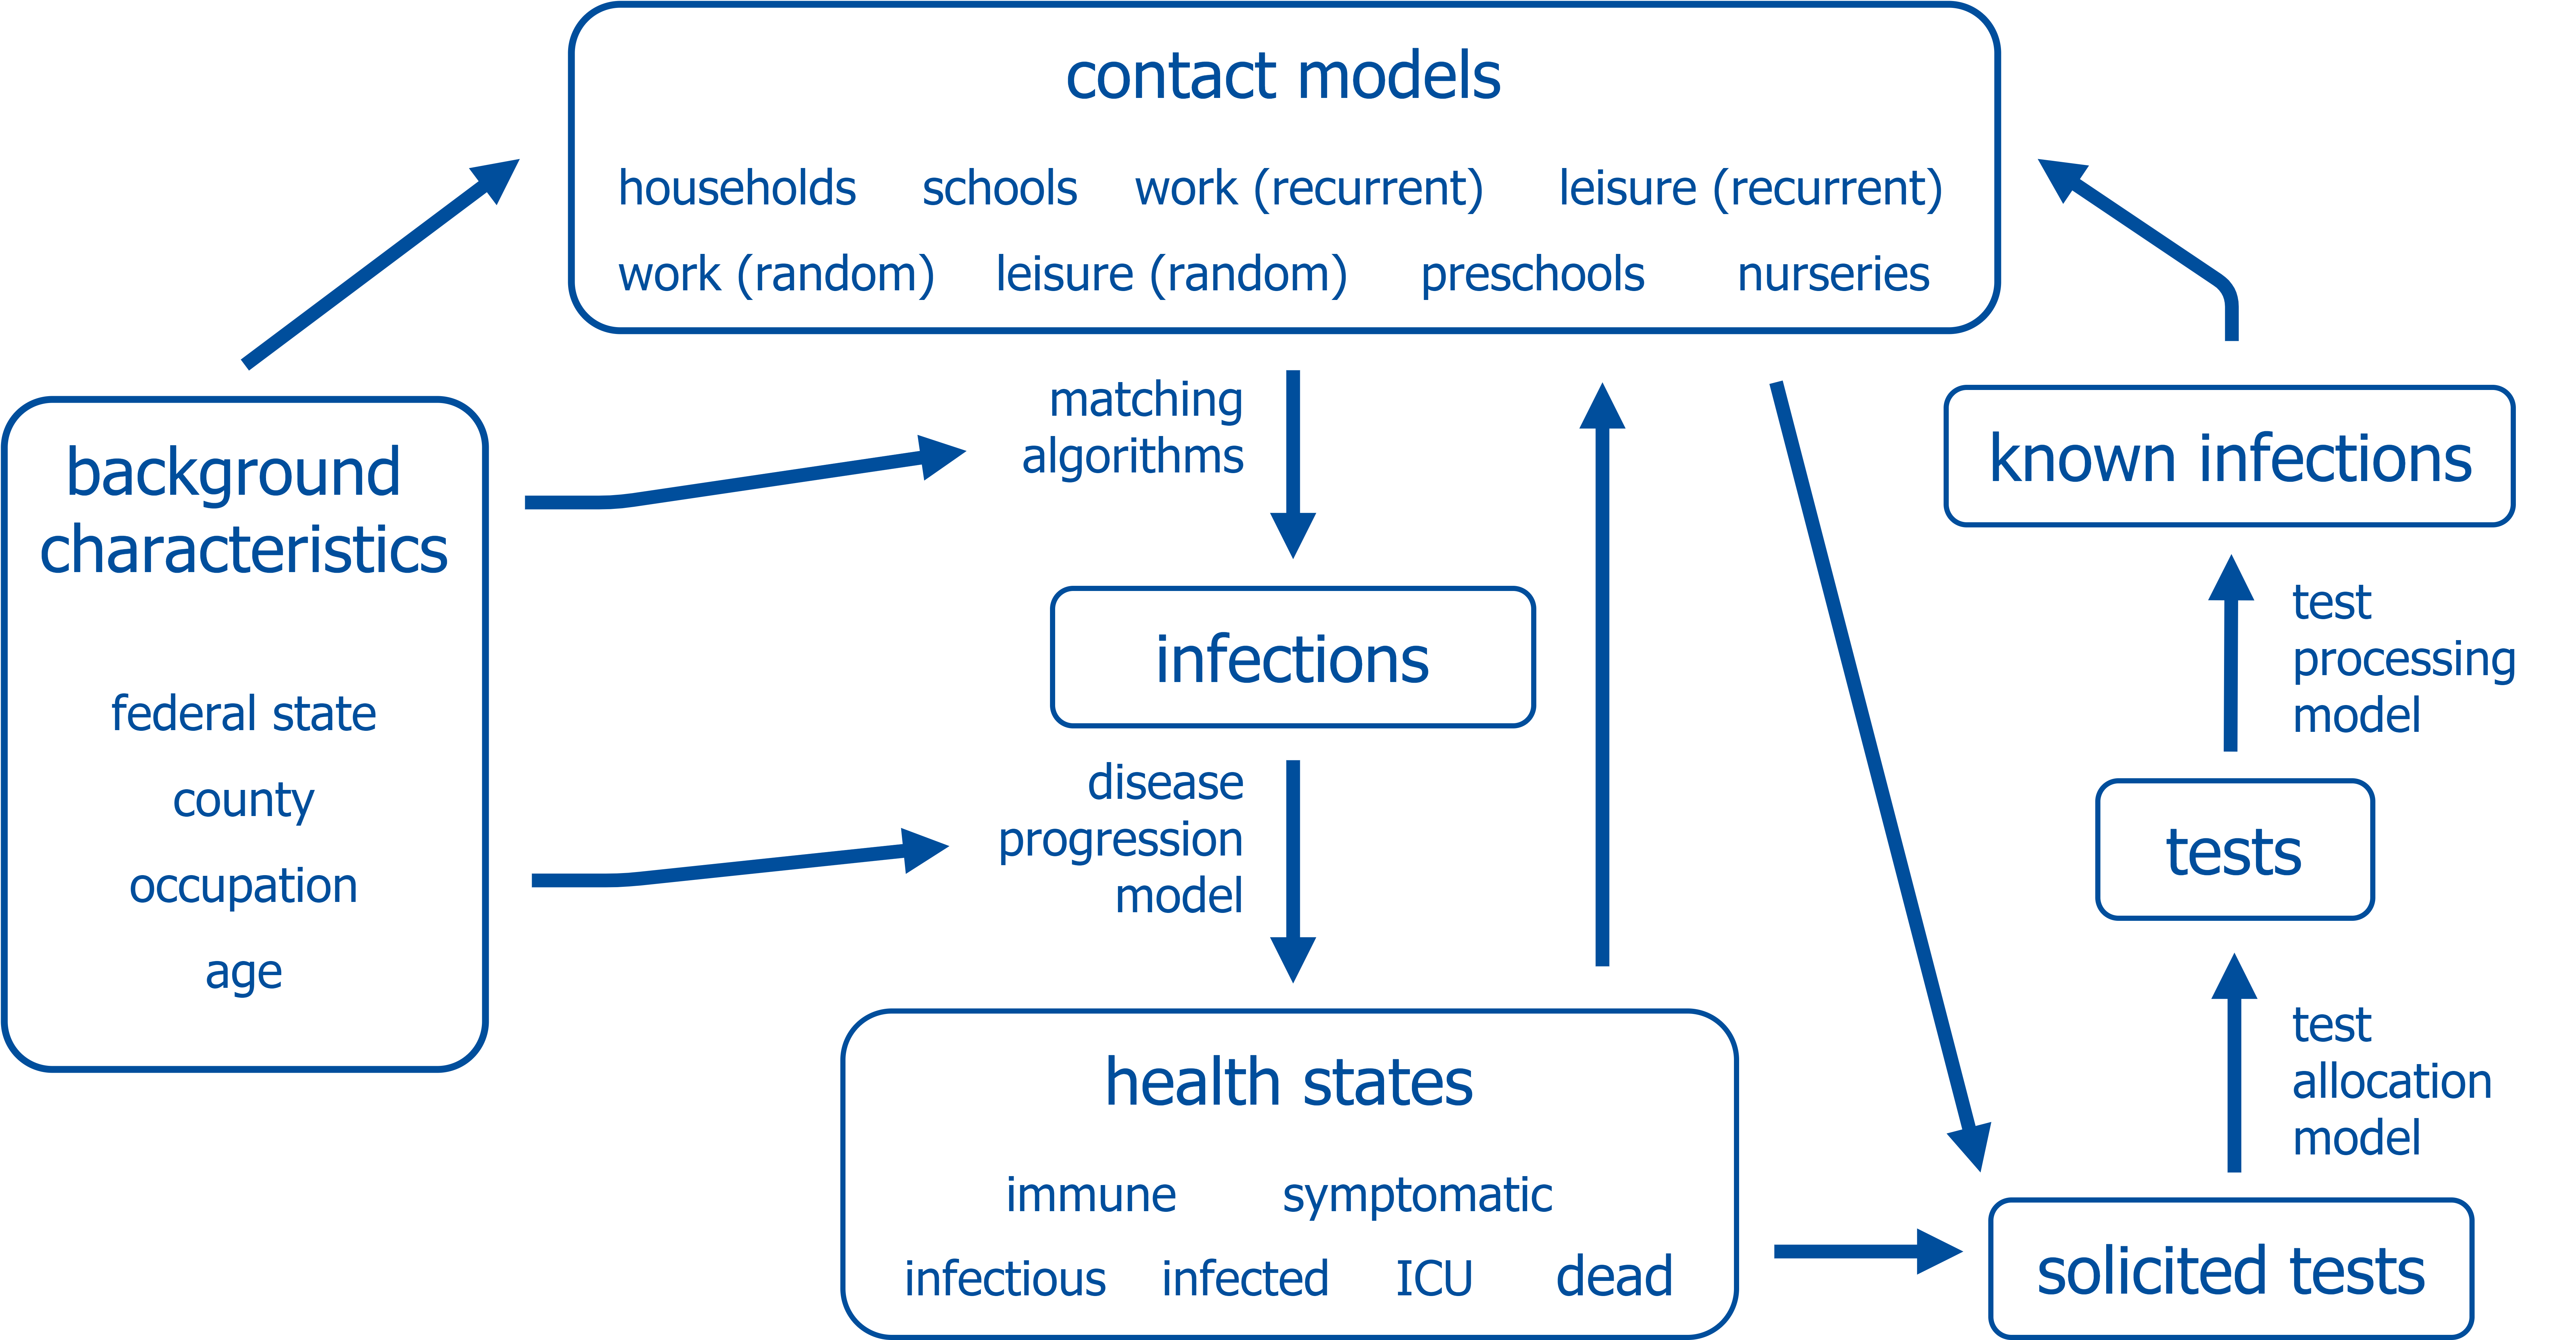
\includegraphics[width=\textwidth]{../figures/model_detailed.png}
        \caption{{\small Model for translating simulated number to officially recorded cases}}
        \label{fig:model_for_official_cases}
    \end{subfigure}

    \caption{Model description}
    \label{fig:model-description}
\end{figure}

Susceptibility to contracting the SARS-CoV-2 virus is dependent on age; so is the progression of a possible infection. We differentiate between an inital period of infection without being infectious or showing symptoms, being infectious (presymptomatic or asymptomatic), showing symptoms, requiring intensive care, and recovery or death. The probabilities of transitioning between these states depend on age; their duration is random within intervals calibrated to medical literature.\comment[id=HM]{Cite}. Conditional on the type of contact, infectiousness independent of ages.\comment[id=HM]{Cite current Drosten paper}

The model includes several other features, which are crucial to describe the evolution of the pandemic in 2020-2021. New virus strains with different profiles regarding infectiousness and disease progress can be introduced. With a probability calibrated to XXX\comment[id=HM]{Klara, please add citatiion}, vaccinated agents become immune and they do not transmit the virus. While vaccines are rolled out, priority may depend on age and occupation. Agents may demand two types of tests as described in Figure~\ref{fig:pcr_antigen_tests}. First, polymerase chain reaction (PCR) tests directly reveal whether an individual is infected or not. PCR tests require some time to be processed and there are always aggregate capacity constraints. Second, rapid antigen tests yield immediate results. Specificity and sensitivity of these tests is set according to the XXX data.\comment[id=HM]{subsequent PCR tests, quarantine, work/school}. Demand for rapid tests will depend on policy, e.g., prices, testing requirements before work, attending school, or visiting restaurants and shops.

Modelling a population of agents according to actual demographic characterists means that we can use a wide array of data to identify and estimate the model's many parameters.\footnote{See section S.X of the supplementary materials for an overview.}\comment[id=HM]{Need to make a list including symbols, maybe you can fetch the parameters from the model and then we brainstorm re notation?} Mobility data is used to model the reductions in work contacts. School and daycare policies are incorporated directly from official directives. Infection rates by age and geographical region are estimated to match to officially recorded numbers; so is the prevalence of virus strains. In order to translate simulated cases in our model to officially recorded cases, we use the model depicted in Figure~\ref{fig:model_for_official_cases}. \comment[id=HM]{Add a sentence.} A further advantage is that the simulated data have a structure that resembles datasets used for regression models, which allows additional plausibility checks by re-running the same models on the model-generated data.\comment[id=HM]{Only keep if we actually do something like that.}

Model that makes the most of many available data sources to gauge the relative effects in this transition period -- see joint distribution of infections with age, geography. But contacts with age, geography, occupations.

We apply this model to Germany. In March and April 2020, the country broke the first wave of the pandemic fairly quickly. Between mid-May and mid-September, daily new infections were below 20 per Million and day.\comment[id=HM]{Cite our world in data} We model the period mid-September 2020 to the end of May 2020. We pick the starting date for two reasons. First, we do not include the first wave because the environment was very different (e.g., aggregate PCR test capacity was much lower and we would require a very different model for calculating the share of known cases) and some data was not recorded yet.\comment[id=HM]{True?}. Second, a large fraction cases during summer of 2020 were traced to international travel,\comment[id=HM]{citation?}, but the precise number is difficult to model.

Figure~\ref{fig:pandemic_drivers_model_fit} describes the evolution of the pandemic and of its drivers. The black line in Figure~\ref{fig:aggregated_fit} shows officially recorded cases; the \replaced[id=HM]{color}{blue?} line in Figure~\ref{fig:stringency_index} the Oxford Response Stringency Index\cite{Hale2020}, which tracks the tightness of non-pharmaceutical interventions. We transform the index so that lower values represent higher levels of restrictions. A value of zero means all measures incorporated in the index are turned on. The value 1 represents the situation of mid-September, where half of all restrictions incorporated in the index are active.\comment[id=HM]{Need to find version of index with a couple of measures, probably need the API access...}. In the six weeks between mid September and mid October, cases increased by a factor of \replaced[id=HM]{X}{10? Do we have RKI numbers as table somewhere?}. Restrictions were somewhat tightened in mid-October and again in early November. New infections remained constant throughout November, before rising again in December.

\begin{figure}[!tp]
    \centering

    \begin{subfigure}[b]{0.475\textwidth}
        \centering
        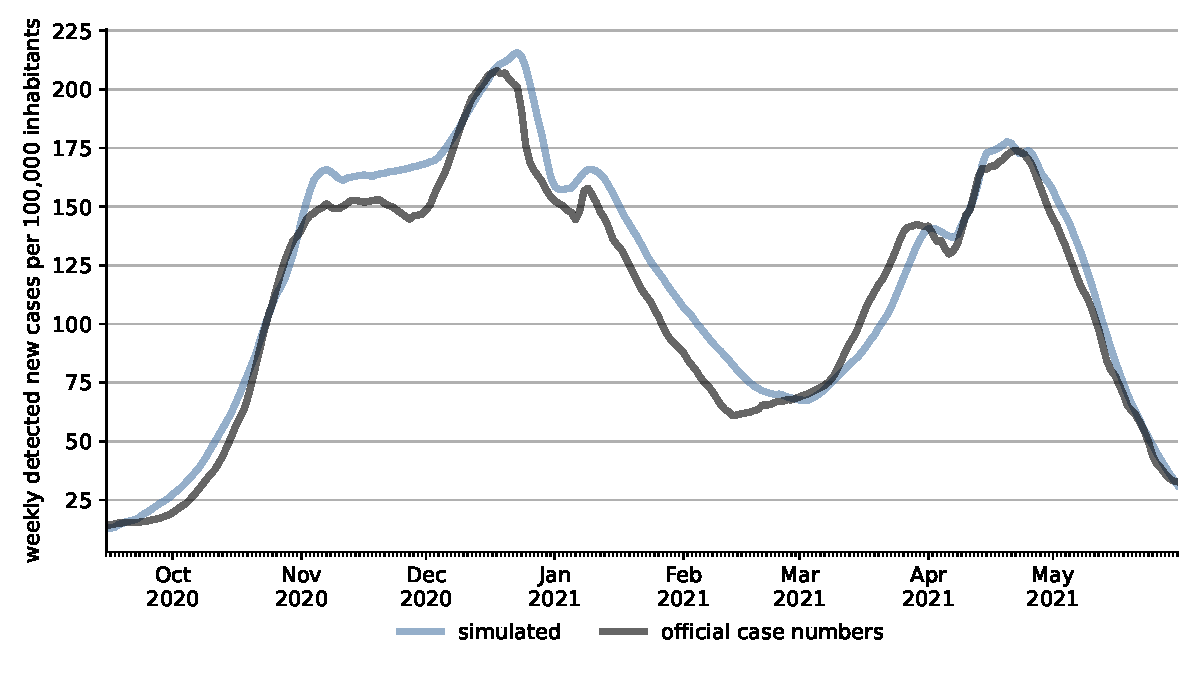
\includegraphics[width=\textwidth]{../figures/results/figures/scenario_comparisons/combined_fit/full_new_known_case}
        \caption{{\small Recorded cases: Empirical and simulated}}
        \label{fig:aggregated_fit}
    \end{subfigure}
    \hfill
    \begin{subfigure}[b]{0.475\textwidth}
        \centering
        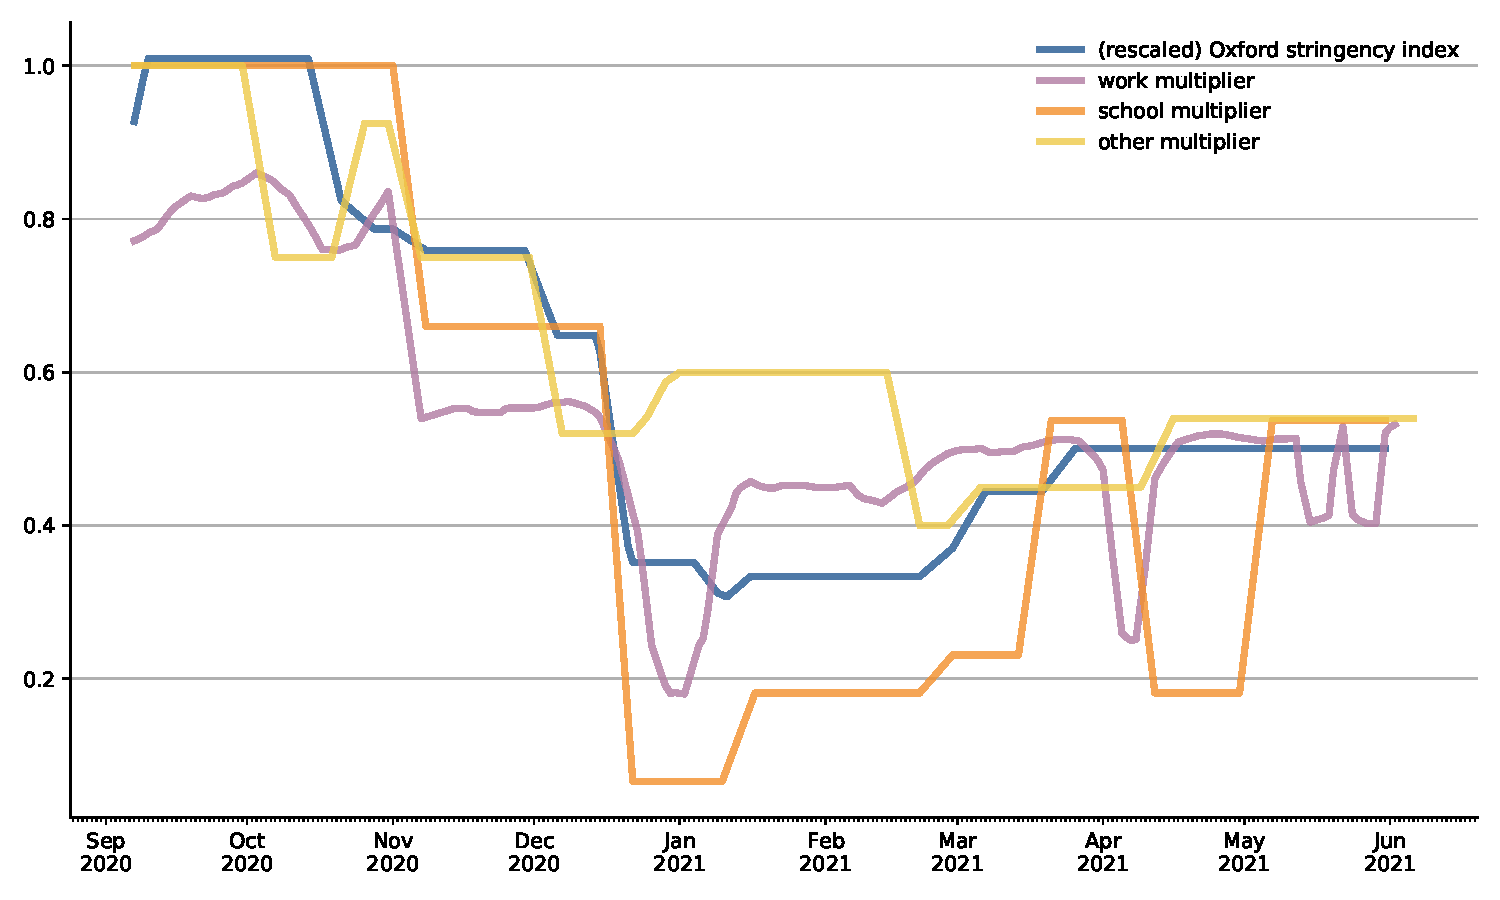
\includegraphics[width=\textwidth]{../figures/results/figures/data/stringency2}

        \caption{{\small Stringency of NPIs and changes in infectious contacts by type}}
        \label{fig:stringency_index}
    \end{subfigure}

    \vskip3ex

    \begin{subfigure}[b]{0.475\textwidth}
        \centering

        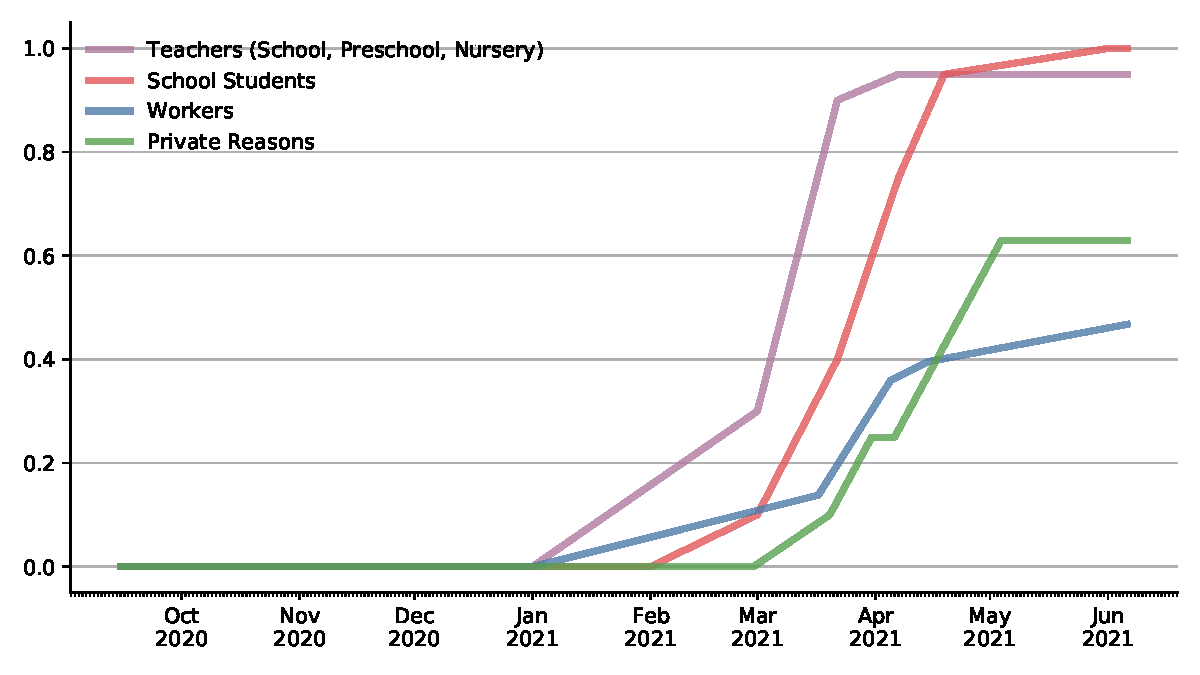
\includegraphics[width=\textwidth]{../figures/results/figures/data/testing/rapid_test_demand_shares}

        \caption{{\small Tests and vaccinations}}
        \label{fig:antigen_tests_vaccinations}
    \end{subfigure}
    \hfill
    \begin{subfigure}[b]{0.475\textwidth}
        \centering
        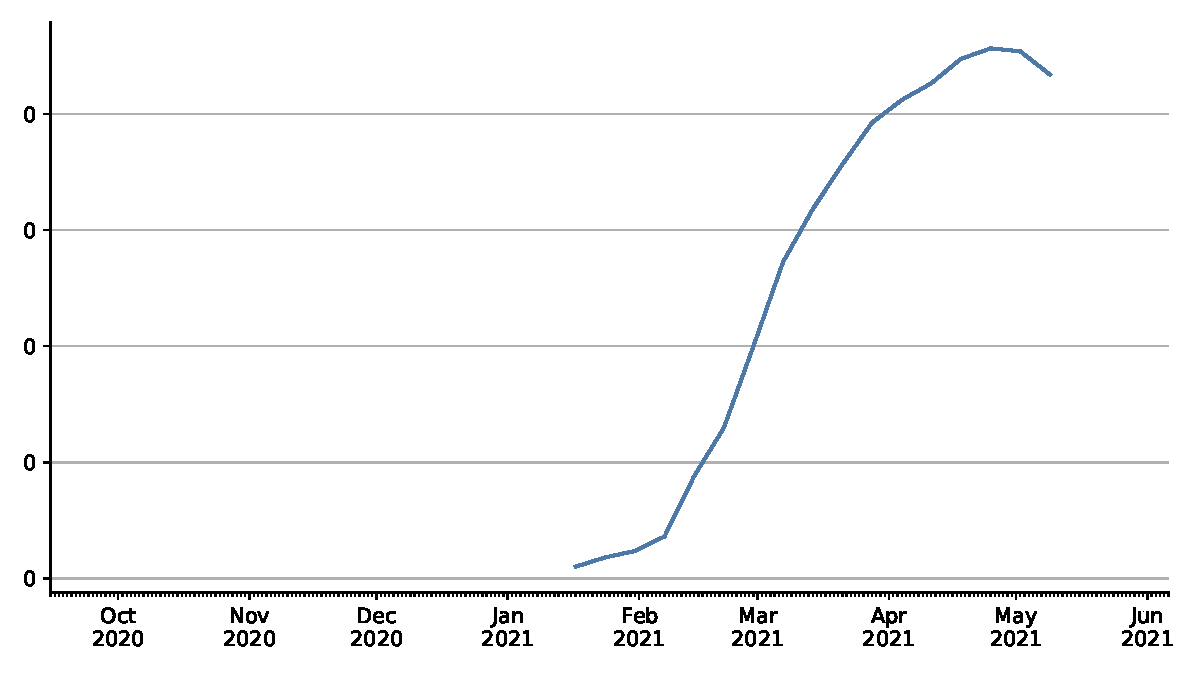
\includegraphics[width=\textwidth]{../figures/results/figures/data/share_of_b117_acc_to_rki}

        \caption{Fraction of B.1.1.7 strain among measured infections}
        \label{fig:share_b117}
    \end{subfigure}

    \caption{Evolution of the pandemic, its drivers, and model fit, September 2020 to May 2021}
    \label{fig:pandemic_drivers_model_fit}

    \floatfoot{
        Note: All aggregates; See S.XXX for statistics by age group and by geographical region. Also more disaggregated data.
    
        Sources: ... 
    }

\end{figure}

Quickly rising rates in December prompted the most stringent lockdown to this date. Schools and daycare centers were closed again, so were customer-facing businesses except for grocery and drug stores. Shortly afterwards, more factors become relevant. Just after Christmas, the first people were vaccinated with a focus on older age groups and medical personnel (Figure~\ref{fig:antigen_tests_vaccinations}. By the end of May, just over 40\% had received at least one dose of a vaccine. Starting in January, rapid tests \dots These had to be administered by medical doctors or in pharmacies. At-home tests approved by authorities were ... in March.\comment[id=HM]{update precise timeline}
From the peak of the second wave just before Christmas until the trough in mid-February, newly detected cases decreased by almost three quarters. The third wave in the spring of 2021 is associated with a rise in the share of the B.1.1.7 variant among all infections, depicted in Figure~\ref{fig:share_b117}, reaching more than 80\% in April\comment[id=HM]{Do we have the table somewhere?}. In early March, some NPIs were being relaxed; e.g., hairdressers and home improvement stores were allowed to open again to the public. In some cases, customers were only allowed to enter with a recent negative rapid test result. 

The blue line in Figure~\ref{fig:aggregated_fit} shows the simulated infections based on our model.

Our model:
\begin{itemize}
    \item Fit is great
    \item Multipliers for three categories (how calculated precisely, refer to appendix for breakdown)
    \item Tests fit well
    \item Share known cases, how calculated
\end{itemize}



Reassured by good fit and a couple of external checks (fall vacation regression?), we consider the relative effects of different measures in 2021
\begin{itemize}
    \item Rapid tests,
    \item seasonality
    \item vaccines
\end{itemize}

lessons learned


\begin{figure}[!tp]
    \centering

    \begin{subfigure}[b]{0.475\textwidth}
        \centering
        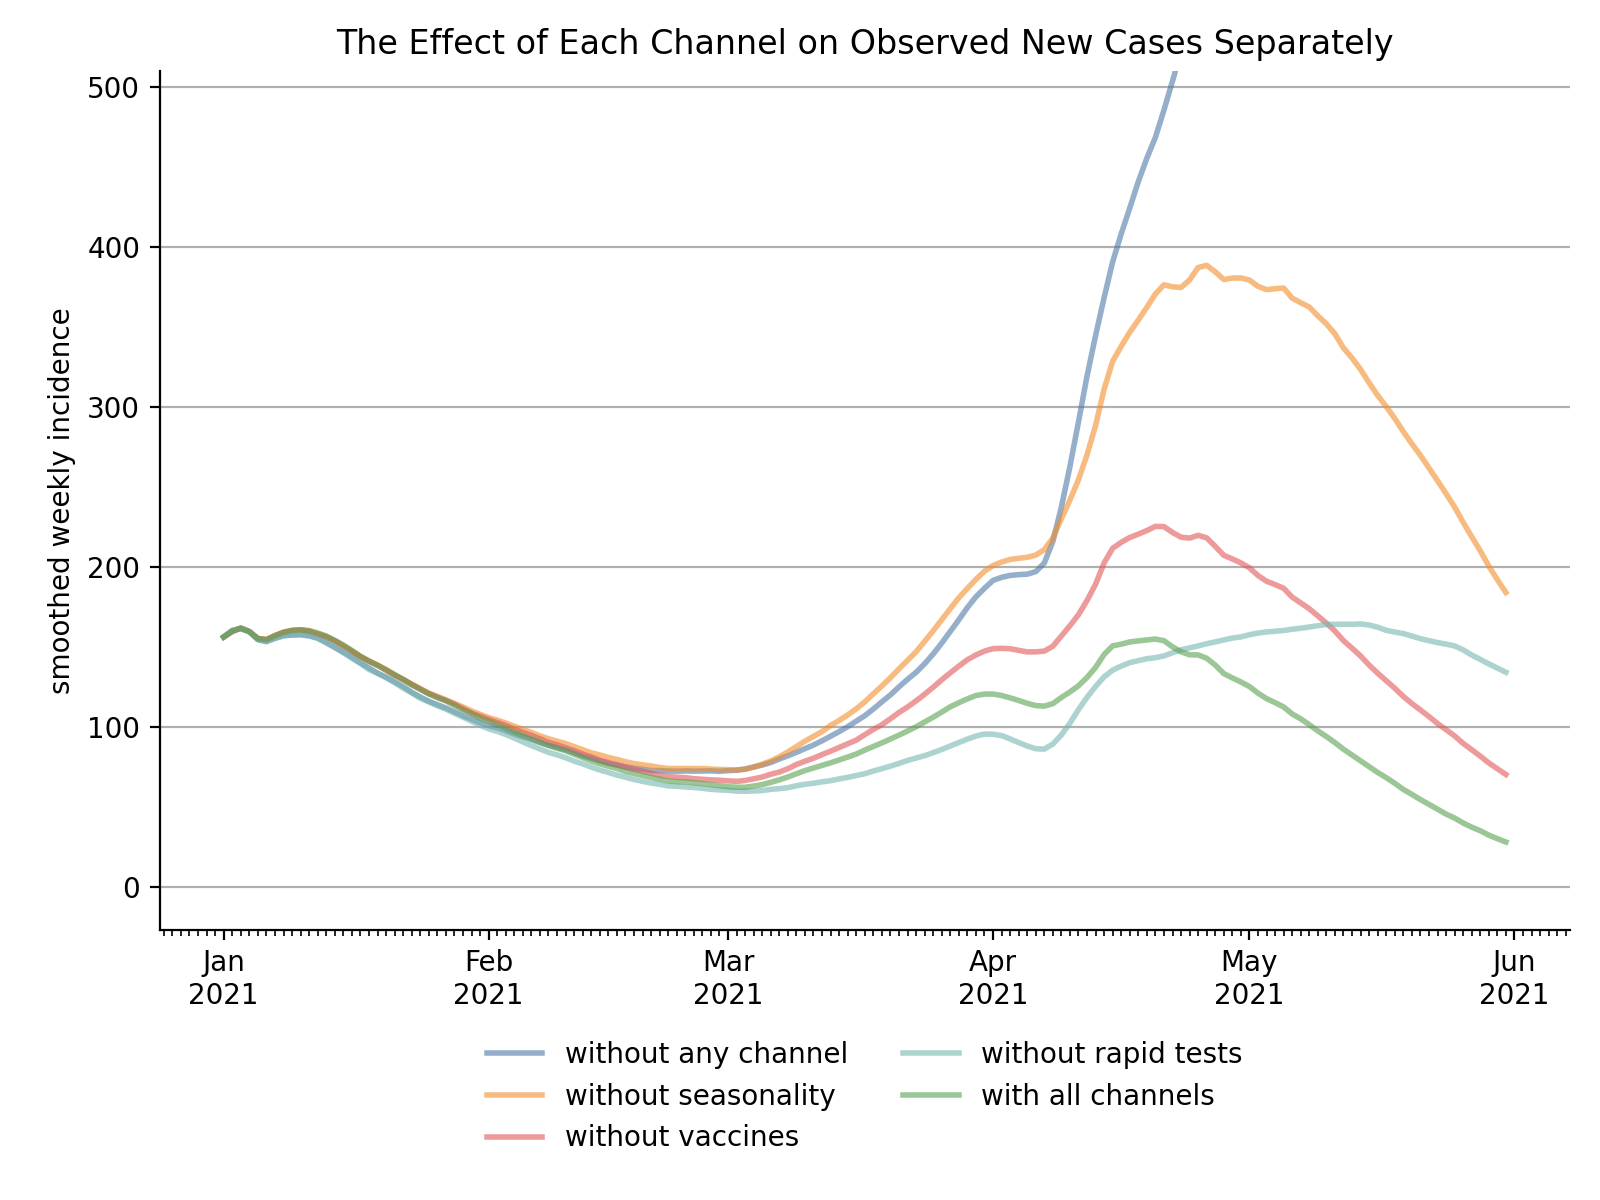
\includegraphics[width=\textwidth]{../figures/results/figures/scenario_comparisons/one_off_and_combined/full_new_known_case_cropped}
        \caption{{\small Recorded cases: 2021 scenarios}}
        \label{fig:full_new_known_case_cropped}
    \end{subfigure}
    %
    \begin{subfigure}[b]{0.475\textwidth}
        \centering
        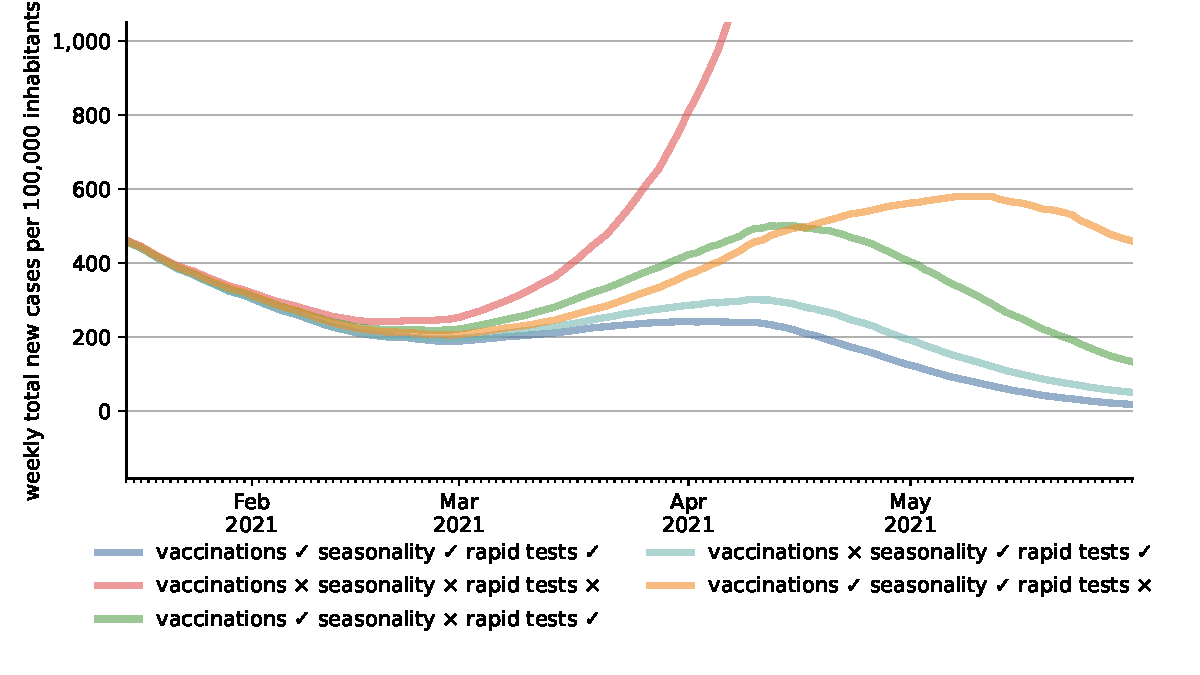
\includegraphics[width=\textwidth]{../figures/results/figures/scenario_comparisons/one_off_and_combined/full_newly_infected_cropped}
        \caption{{\small Total cases: 2021 scenarios}}
        \label{fig:full_newly_infected_cropped}
    \end{subfigure}

    \begin{subfigure}[b]{0.475\textwidth}
        \centering
        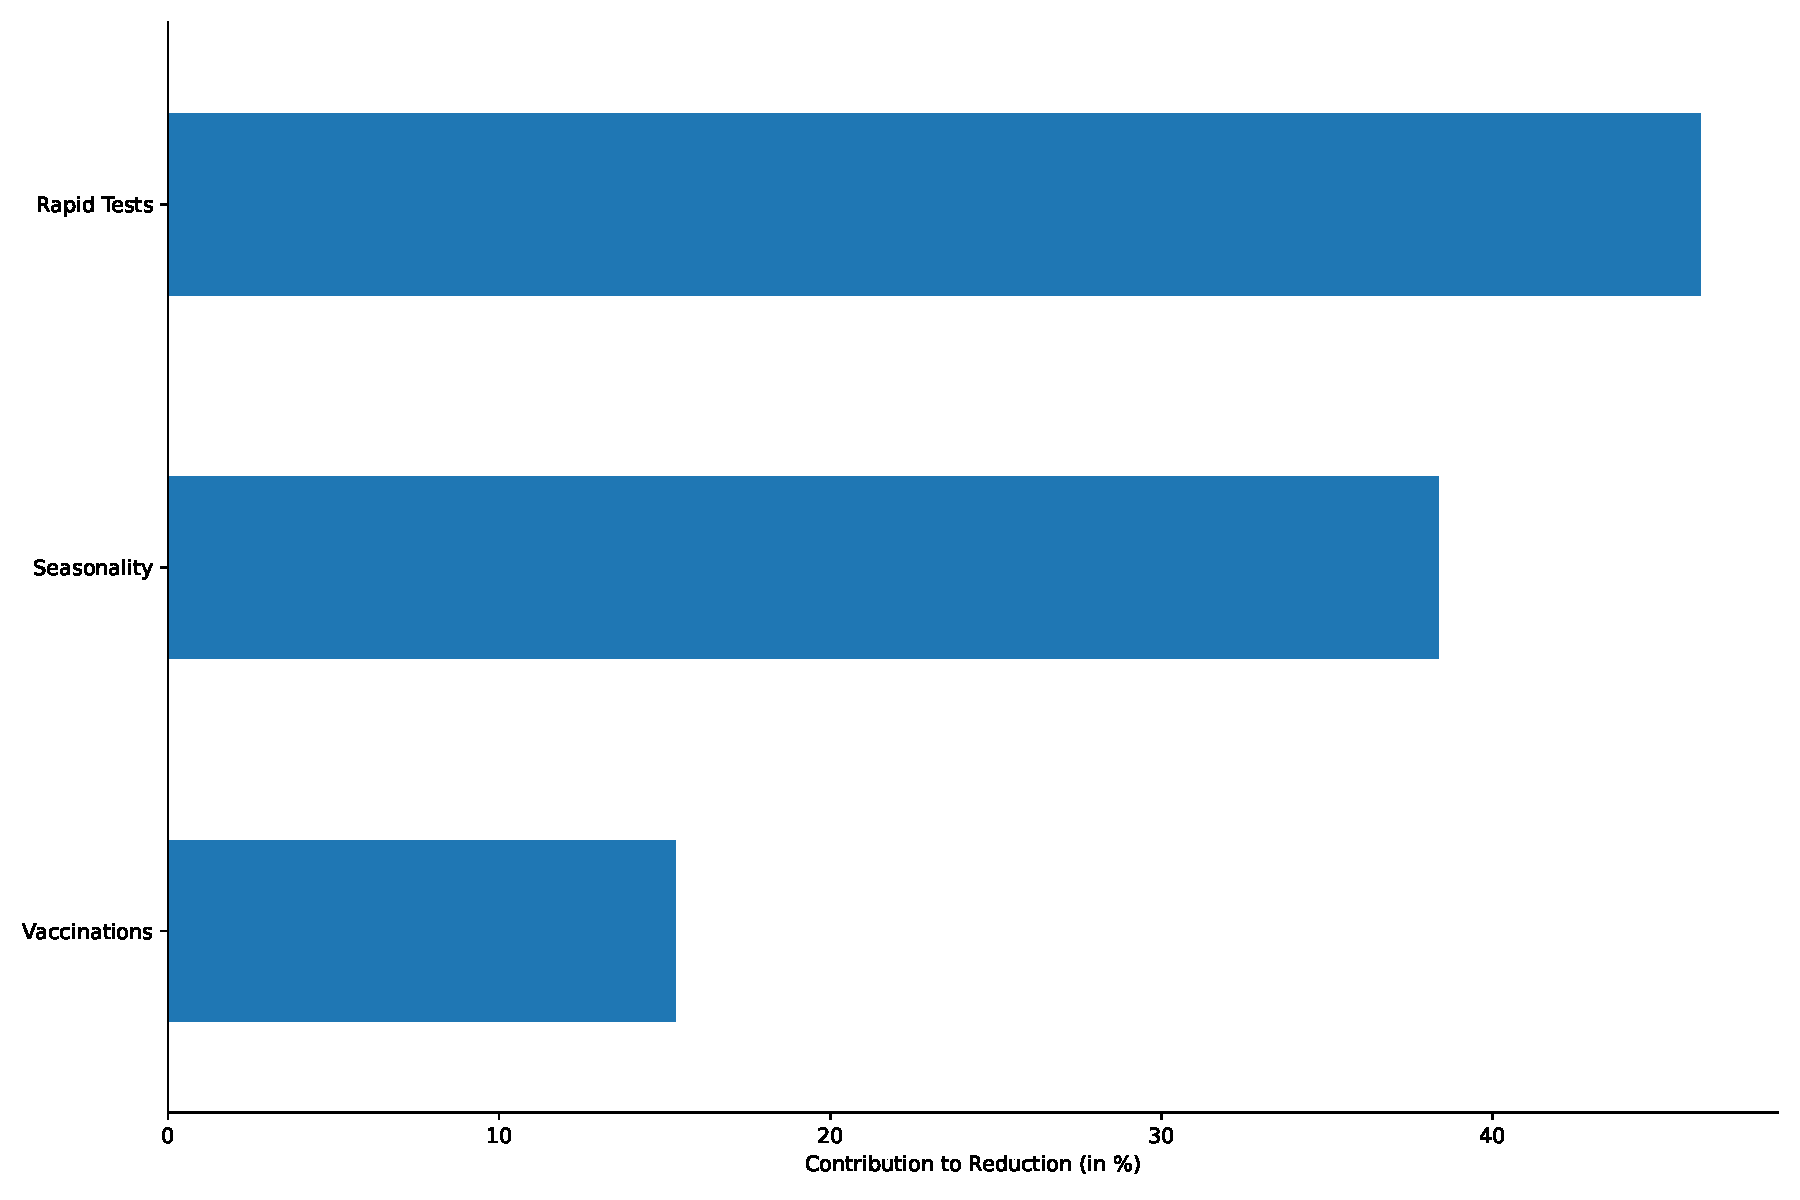
\includegraphics[width=\textwidth]{../figures/full_decomposition}

        \vskip2ex

        \caption{Decomposition of effects for Figure~\ref{fig:full_newly_infected_cropped}.}

        \label{fig:decomposition_scenarios_total_cases}
    \end{subfigure}
    %
    \begin{subfigure}[b]{0.475\textwidth}
        \centering
        
        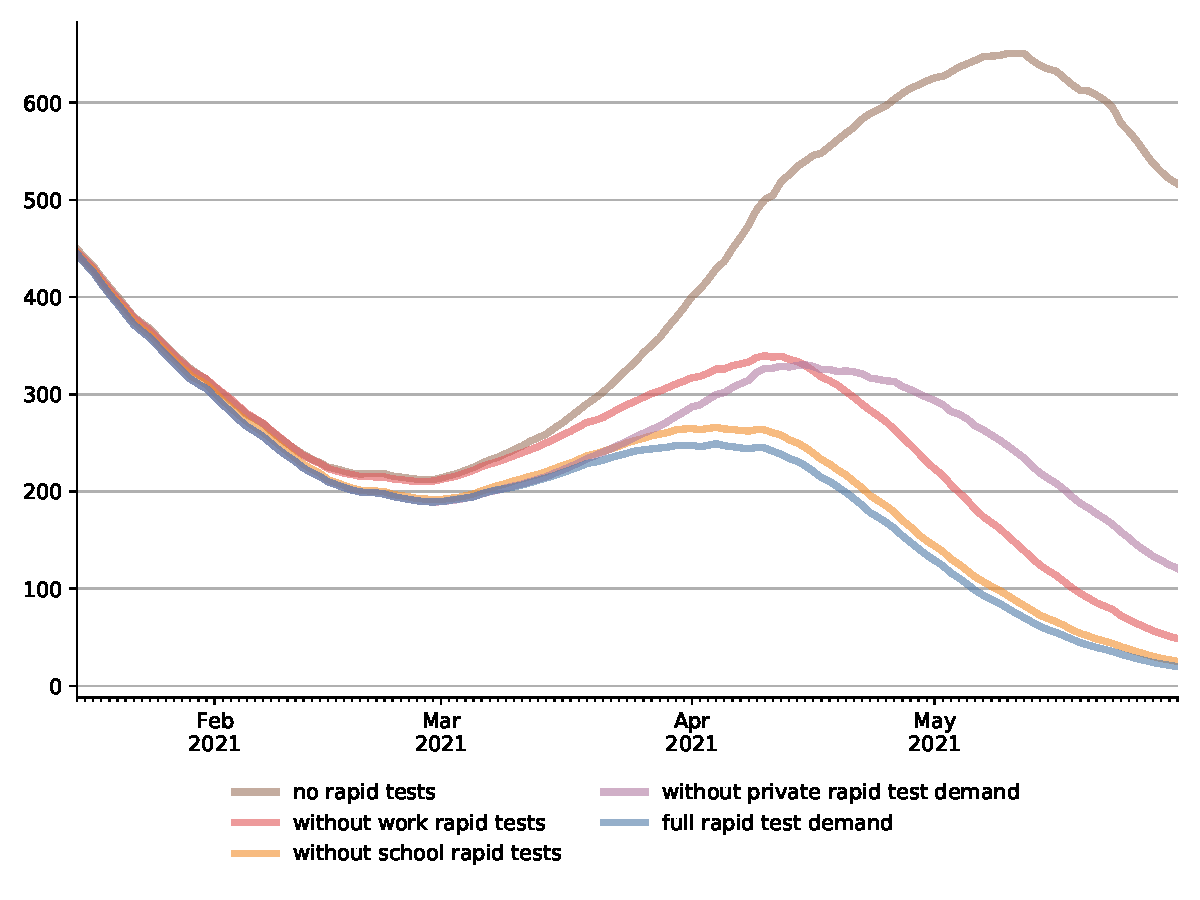
\includegraphics[width=\textwidth]{../figures/results/figures/scenario_comparisons/effect_of_rapid_tests/full_newly_infected}
        \caption{{\small Effects of different types of testing}}
        \label{fig:decomposition_tests}
    \end{subfigure}
    
    \caption{The effect of different interventions on recorded and actual infections}
    \label{fig:interventions_broad}
    
    \floatfoot{
        Note: All aggregates; See S.XXX for statistics by age group and by geographical region.
    
        The decomposition is based on Shapley values where the individual contribution of an intervention is its average contribution over different sizes of coalitions (combinations with other interventions). The individual contribution to a coalition is the difference between the effect size of the coalition with the particular intervention and without.
    }
\end{figure}

Schooling very contentious. Likely damage to child development.

We show

Screening effect: ...


\begin{figure}[!tp]
    \centering

    \begin{subfigure}[b]{0.475\textwidth}
        \centering
        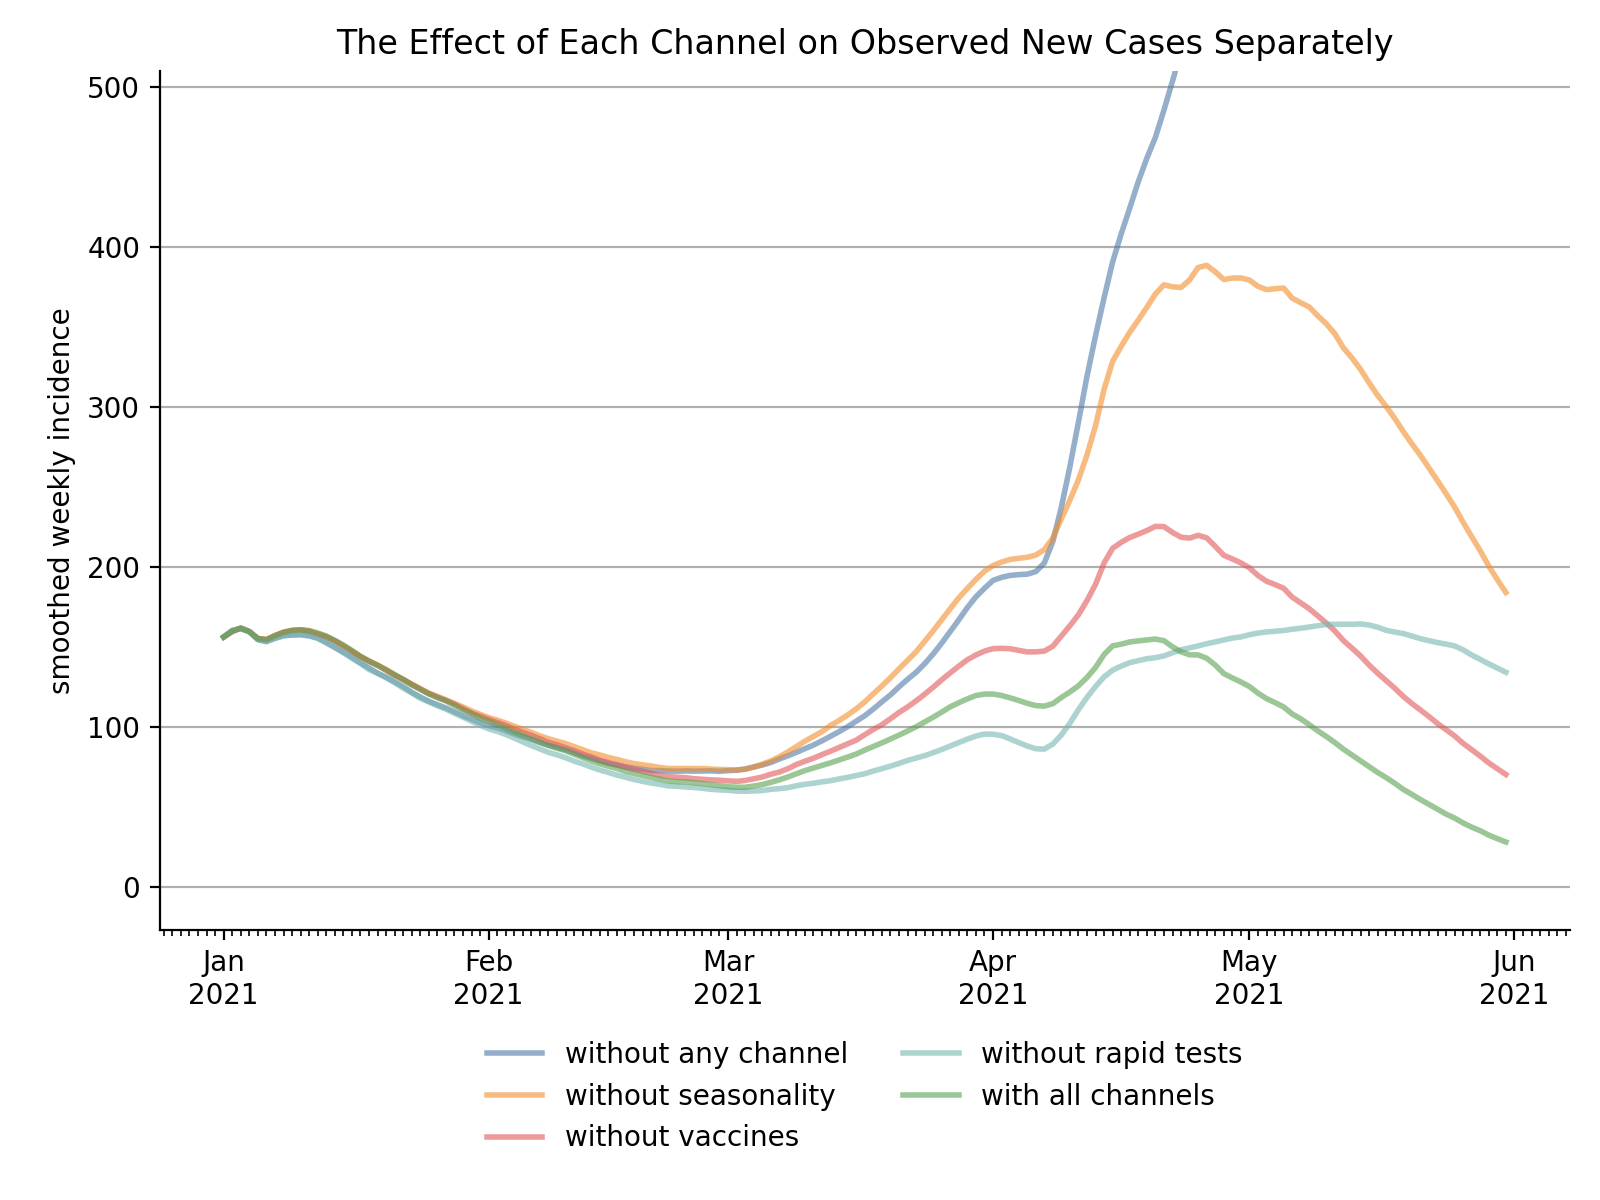
\includegraphics[width=\textwidth]{../figures/results/figures/scenario_comparisons/one_off_and_combined/full_new_known_case_cropped}
        \caption{{\small Effects of different schooling scenarios after Easter}}
        \label{fig:schooling_scenarios_easter}
    \end{subfigure}
    \hfill
    \begin{subfigure}[b]{0.475\textwidth}
        \centering
        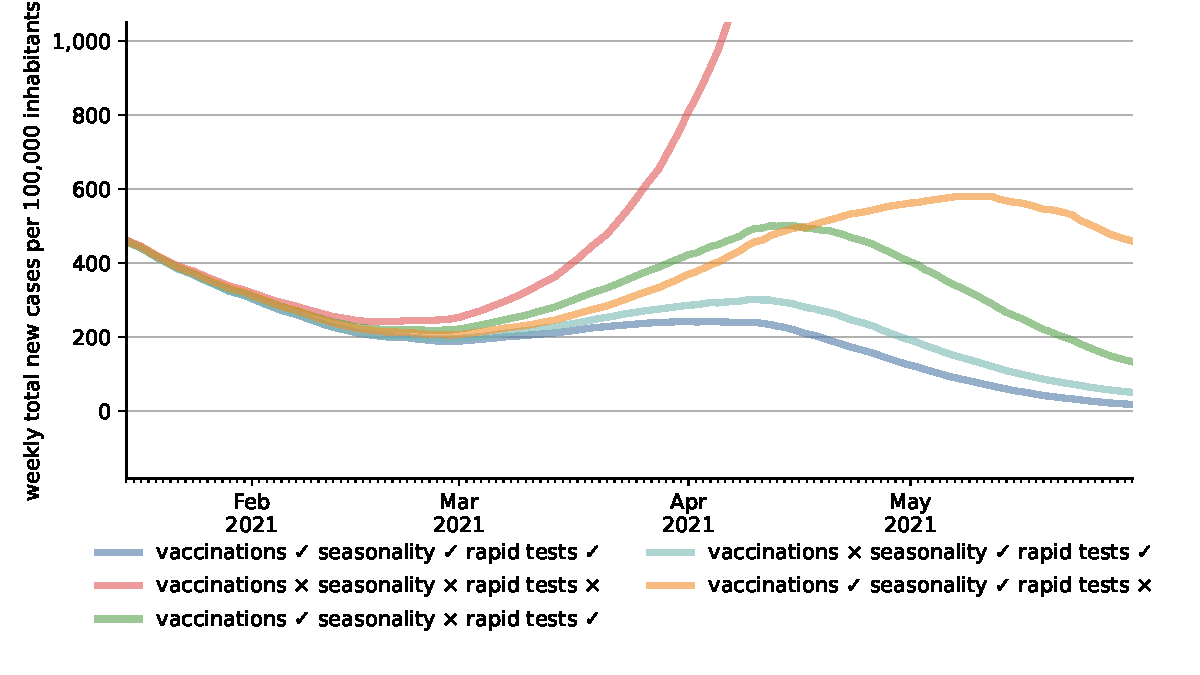
\includegraphics[width=\textwidth]{../figures/results/figures/scenario_comparisons/one_off_and_combined/full_newly_infected_cropped}
        \caption{{\small TBD}}
        \label{fig:to_be_determined}
    \end{subfigure}
    \vskip3ex    

    \caption{Schooling / maybe home office}
    \label{fig:interventions_school}

    Note: All aggregates; See S.XXX for statistics by age group and by geographical region.

\end{figure}




\paragraph{Points to mention}
\begin{itemize}
    \item If anything too optimistic regarding vaccinations
    \item Social structure / conditional block testing in families important (?)
    \item Trump-effect: More testing = more cases true for how long?
\end{itemize}

% Technical terms should be defined. 

% Symbols, abbreviations, and acronyms should be defined the first time they are used. 

% All tables and figures should be cited in numerical order.

% All data must be shown either in the main text or in the Supplementary Materials or must be available in an established database with accession details provided in the acknowledgements section.

% References to unpublished materials are not allowed to substantiate significant conclusions of the paper.


\section{Supplementary Material}

\begin{enumerate}
    \item Model
    \item Data
    \item Identification and Estimation
\end{enumerate}